\section{METODOLOGIA}

A condução deste trabalho divide-se em duas partes complementares e integradas. A primeira parte compreende os procedimentos de pesquisa científica, responsáveis por investigar o problema real do desaparecimento de animais, diagnosticar as necessidades dos tutores e mapear as deficiências das soluções tecnológicas existentes no mercado. A segunda parte estabelece a metodologia de engenharia de software aplicada ao desenvolvimento da aplicação móvel proposta, definindo o modelo de ciclo de vida do sistema, o método ágil de controle de tarefas e as etapas técnicas percorridas desde a concepção inicial até a validação com usuários finais.

\subsection{Metodologia e Procedimentos da Pesquisa}

Para estruturar as decisões de projeto e garantir rigor acadêmico, a pesquisa foi organizada segundo a taxonomia proposta por Gil (2022) e Lakatos e Marconi (2021). Quanto à natureza, classifica-se como pesquisa aplicada, pois visa solucionar um problema prático da sociedade relativo à demora e às dificuldades na localização de animais de estimação desaparecidos, resultando na concepção de uma ferramenta funcional e acessível.

Em relação à abordagem do problema, adota-se um caráter quali-quantitativo integrado. O viés quantitativo envolve a tabulação estatística das respostas obtidas no formulário diagnóstico e a mensuração numérica da usabilidade pelo protocolo SUS. Por sua vez, a dimensão qualitativa compreende a análise das dificuldades relatadas pelos tutores, o estudo crítico das interfaces de sistemas similares e a avaliação das opiniões expressas pelos voluntários durante os testes práticos.

Quanto aos objetivos gerais, o estudo assume perfil exploratório e descritivo. O aspecto exploratório proporcionou maior aproximação com os desafios e sentimentos de angústia enfrentados pelos tutores, ao passo que o caráter descritivo permitiu mapear e correlacionar os canais habituais de divulgação e os recursos das ferramentas concorrentes. Por fim, quanto aos procedimentos técnicos, combinou-se o levantamento bibliográfico em livros, artigos e normas técnicas, a pesquisa de campo mediante questionário estruturado com tutores e protetores, e a análise comparativa direta sobre plataformas existentes no mercado.

\subsubsection{Pesquisa de Viabilidade com a Comunidade (Levantamento de Campo)}

A coleta primária de dados foi realizada por meio de um questionário estruturado online elaborado na plataforma Google Forms (cujo instrumento estruturado encontra-se documentado na íntegra no Apêndice B, Seção B.1), submetido a 20 participantes voluntários, incluindo tutores de animais domésticos, protetores independentes e pessoas engajadas na causa animal.

O formulário iniciou investigando os hábitos preventivos de identificação animal adotados pelos tutores no cotidiano, consultando os voluntários a respeito do uso de microchips eletrônicos em seus animais de estimação, conforme ilustrado na Figura~\ref{fig:adocao_microchip}.

\begin{figure}[H]
    \centering
    \caption{Adesão ao uso de microchip de identificação em animais domésticos}
    \label{fig:adocao_microchip}
    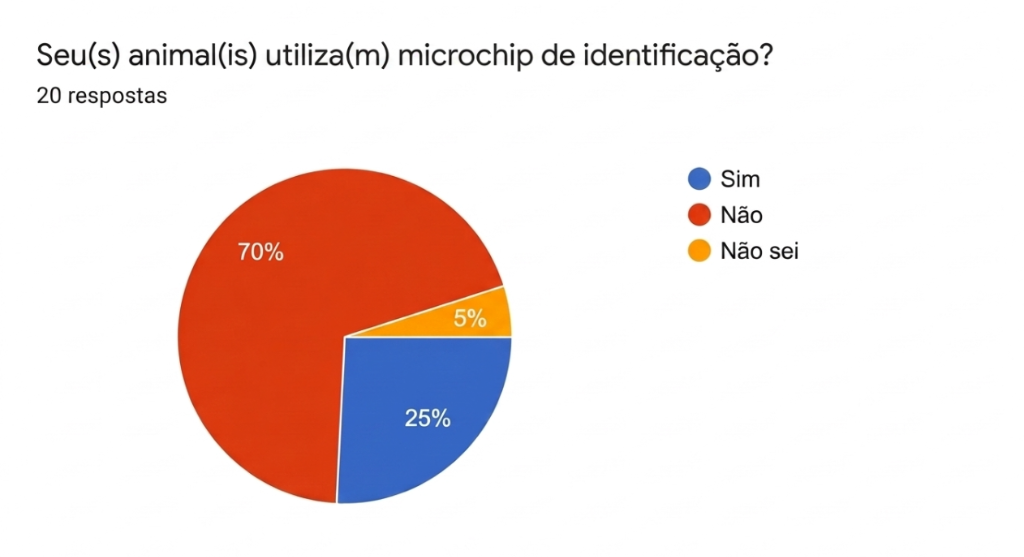
\includegraphics[width=0.90\textwidth]{imagens/01_pesquisa/grafico_adocao_microchip.png}
    \fonte{Dados da pesquisa (Google Forms, 2026)}
\end{figure}

Os dados da Figura~\ref{fig:adocao_microchip} revelam que a expressiva maioria dos animais (70\%, totalizando 14 respostas) não utiliza microchip de identificação, somando-se a 5\% (1 resposta) de participantes que declararam não saber responder. Apenas 25\% dos respondentes (5 participantes) afirmaram que seus animais são microchipados, evidenciando uma baixa adesão a esse método de identificação entre os participantes da pesquisa.

Em paralelo à identificação eletrônica interna, o questionário avaliou os métodos externos e visuais empregados pelos tutores no cotidiano, investigando a utilização de coleiras de identificação (Figura~\ref{fig:uso_coleira}).

\begin{figure}[H]
    \centering
    \caption{Utilização de coleiras de identificação em animais domésticos}
    \label{fig:uso_coleira}
    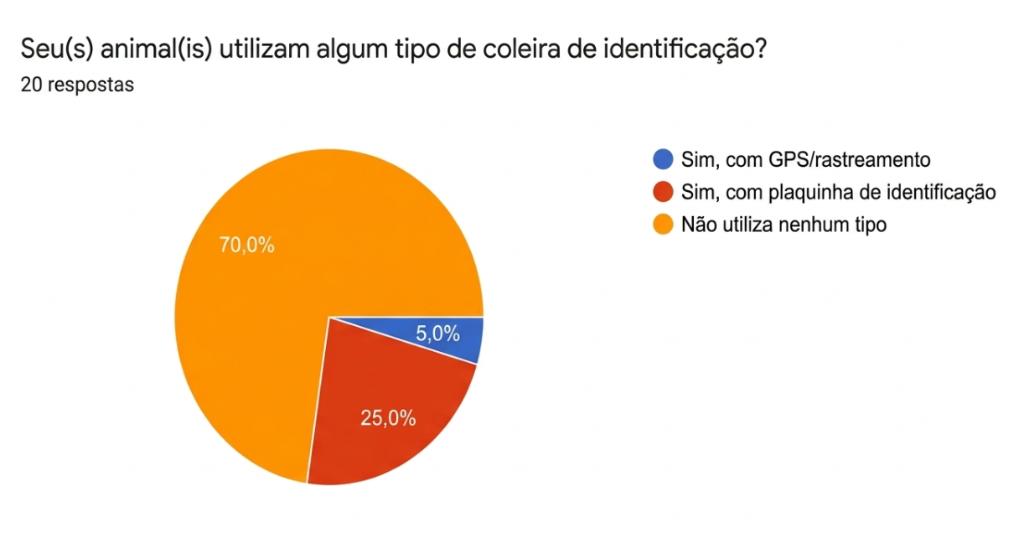
\includegraphics[width=0.90\textwidth]{imagens/01_pesquisa/grafico_uso_coleira.png}
    \fonte{Dados da pesquisa (Google Forms, 2026)}
\end{figure}

Conforme ilustrado na Figura~\ref{fig:uso_coleira}, a expressiva maioria dos entrevistados (70\%, totalizando 14 respostas) indicou que seus animais não utilizam nenhum tipo de coleira de identificação. Entre os que adotam algum recurso, 25\% (5 respostas) utilizam plaquinha de identificação convencional e apenas 5\% (1 resposta) contam com coleira equipada com GPS ou rastreamento. Os dados revelam que a maior parte dos animais circula sem qualquer forma externa de identificação visual.

Na sequência, o questionário mapeou o comportamento prático dos participantes durante episódios reais de desaparecimento, identificando os canais digitais e analógicos mais acionados para a divulgação da ocorrência. A Figura~\ref{fig:pesquisa_meios} apresenta os meios habituais de busca apontados pelos voluntários.

\begin{figure}[H]
    \centering
    \caption{Meios habituais de divulgação utilizados em episódios de animais perdidos}
    \label{fig:pesquisa_meios}
    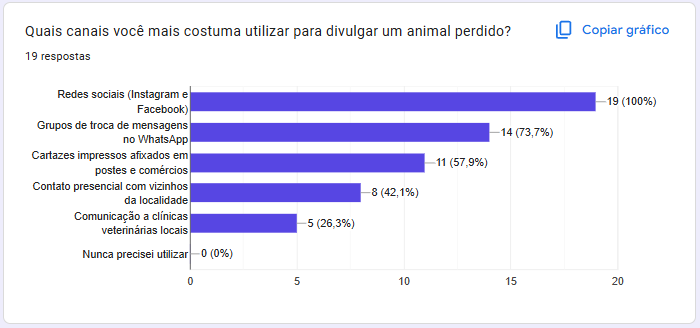
\includegraphics[width=0.90\textwidth]{imagens/01_pesquisa/figura01_canais_divulgacao.png}
    \fonte{Dados da pesquisa (Google Forms, 2026)}
\end{figure}

Os dados da Figura~\ref{fig:pesquisa_meios} indicam que a quase totalidade dos participantes concentra seus esforços nas redes sociais convencionais (11 respostas, equivalentes a 55\%) e nos grupos de troca de mensagens do WhatsApp (5 respostas, ou 25\%). Em contrapartida, as mídias impressas tradicionais, a exemplo de cartazes fixados em postes e comércios locais, somaram apenas 2 escolhas (10\%), ao passo que a busca presencial com vizinhos e avisos em clínicas veterinárias representaram 5\% cada.

Apesar da ampla utilização das redes sociais genéricas, os participantes relataram obstáculos críticos: as postagens perdem alcance aceleradamente devido ao fluxo contínuo de novas publicações no feed, não há filtros espaciais que limitem o aviso ao bairro do desaparecimento e dados cruciais dispersam-se em comentários paralelos.

Para solucionar esse problema de alcance e dispersão geográfica, avaliou-se o interesse dos voluntários em relação a uma aplicação móvel dedicada que integrasse mapa georreferenciado por GPS e filtros de proximidade. O resultado está ilustrado na Figura~\ref{fig:interesse_mapa}.

\begin{figure}[H]
    \centering
    \caption{Nível de interesse e aceitação do mapa interativo e recursos de proximidade}
    \label{fig:interesse_mapa}
    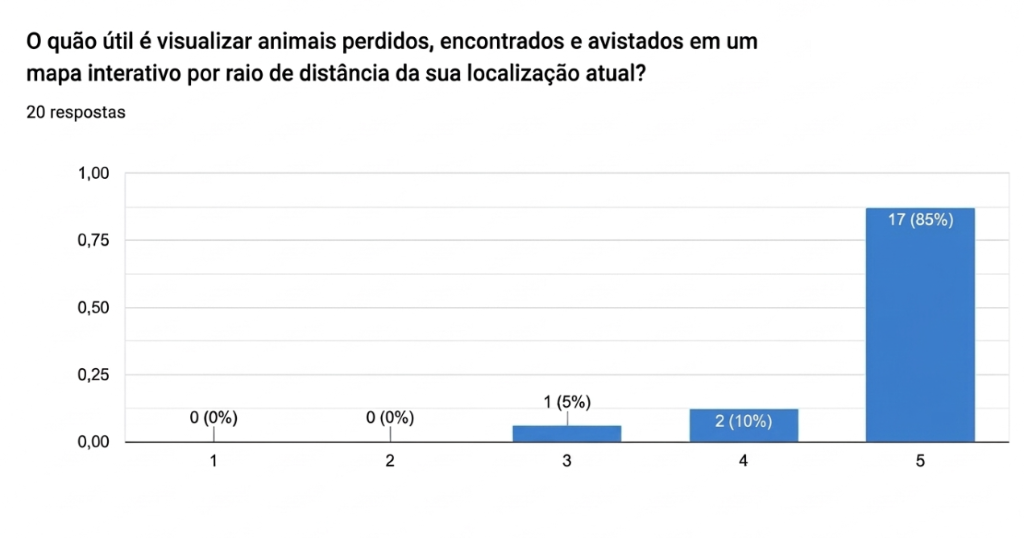
\includegraphics[width=0.90\textwidth]{imagens/01_pesquisa/figura02_interesse_mapa.png}
    \fonte{Dados da pesquisa (Google Forms, 2026)}
\end{figure}

A aceitação verificada na Figura~\ref{fig:interesse_mapa} foi amplamente favorável: 17 participantes (85\%) atribuíram nota máxima 5 à utilidade do mapa interativo com filtro de proximidade, 2 participantes (10\%) indicaram nota 4 e apenas 1 participante (5\%) atribuiu nota 3, sem nenhum registro de notas 1 ou 2. Esse resultado demonstra que 95\% dos voluntários consideram a visualização em mapa de extrema utilidade, evidenciando a carência de uma solução tecnológica gratuita e dedicada à causa do reencontro.

\subsubsection{Análise Comparativa de Sistemas Similares}

Para conhecer as soluções existentes e identificar pontos de melhoria para o projeto, realizou-se uma análise comparativa com base nos critérios de usabilidade e experiência do usuário propostos por Amstel (2024). Foram analisadas quatro plataformas representativas da área: \textit{Viu Meu Pet}, \textit{PawBoost}, \textit{AlertPet} e \textit{Pet911}.

\noindent\textbf{Viu Meu Pet:} Trata-se de uma das plataformas brasileiras mais difundidas na área, oferecendo portal web e aplicativo móvel (Figura~\ref{fig:viumeupet}). 

\begin{figure}[H]
    \centering
    \caption{Interface da plataforma Viu Meu Pet}
    \label{fig:viumeupet}
    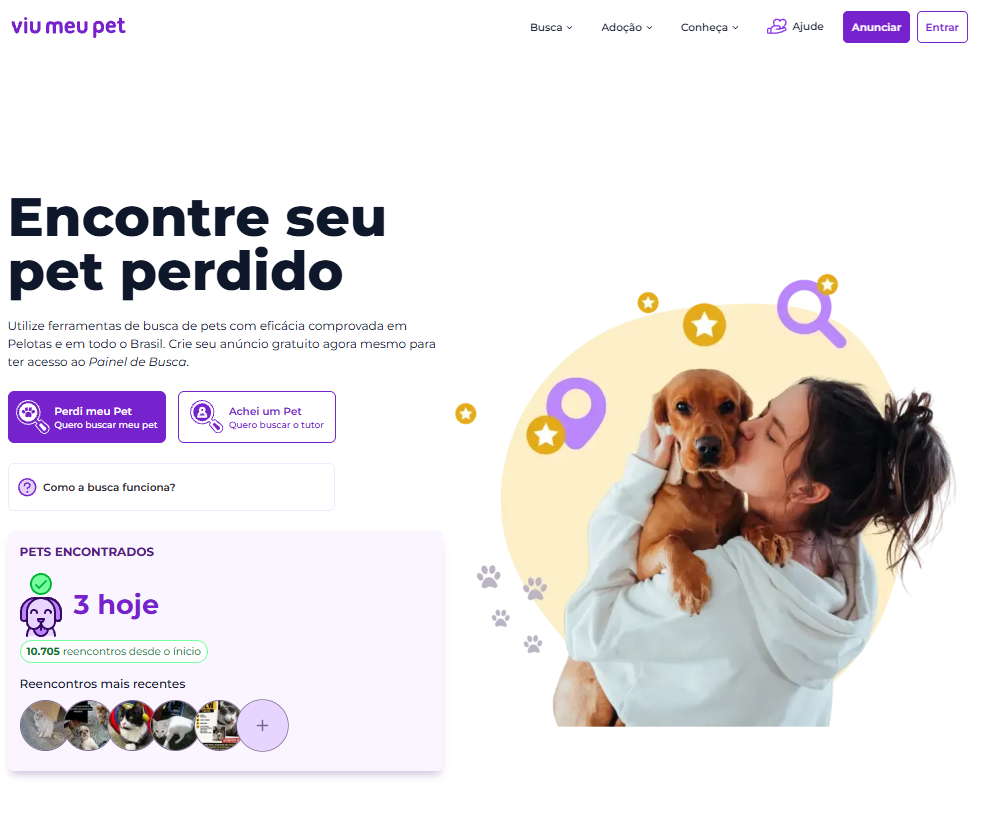
\includegraphics[width=0.90\textwidth]{imagens/01_pesquisa/figura03_viumeupet.png}
    \fonte{Viu Meu Pet (2026)}
\end{figure}

A interface inicial da plataforma (Figura~\ref{fig:viumeupet}) exibe em seu topo o logotipo institucional acompanhado por links de navegação rápida (``Busca'', ``Adoção'' e ``Conheça''), o botão de apoio comunitário (``Ajude''), o botão roxo destacado para inserção de anúncios (``Anunciar'') e o atalho para login (``Entrar''). O corpo central destaca a chamada principal ``Encontre seu pet perdido'' seguida de dois botões primários de triagem: ``Perdi meu Pet (Quero buscar meu pet)'' com fundo roxo e ``Achei um Pet (Quero buscar o tutor)'' com contorno, além do link explicativo ``Como a busca funciona?''. No canto inferior esquerdo, um cartão apresenta métricas em tempo real sob o título ``Pets Encontrados'', indicando ``3 hoje'' e ``10.705 reencontros desde o início'', ao lado de fotografias em miniatura dos animais resgatados. À direita, uma ilustração fotográfica reforça a conexão afetiva entre tutor e animal.

Como pontos positivos, o sistema possui ampla visibilidade comunitária no Brasil, disponibiliza recursos gratuitos como painel de busca, gerador de imagens para redes sociais, cartazes com código QR para impressão e cruzamento automático de anúncios por inteligência artificial, além de serviços pagos de destaque. No entanto, sua navegação é centrada em listagens estáticas separadas por estado e cidade, sem integração fluida com mapa georreferenciado em tempo real por GPS. Outro problema crítico reside na comunicação: a plataforma não oferece chat interno privativo, expondo números particulares de telefone em anúncios públicos.

\noindent\textbf{PawBoost:} Plataforma internacional com mais de sete milhões de membros cadastrados em sua rede de voluntários (\textit{Rescue Squad}™), acessível via web e aplicativos para Android e iOS (Figura~\ref{fig:pawboost}).

\begin{figure}[H]
    \centering
    \caption{Interface da plataforma PawBoost}
    \label{fig:pawboost}
    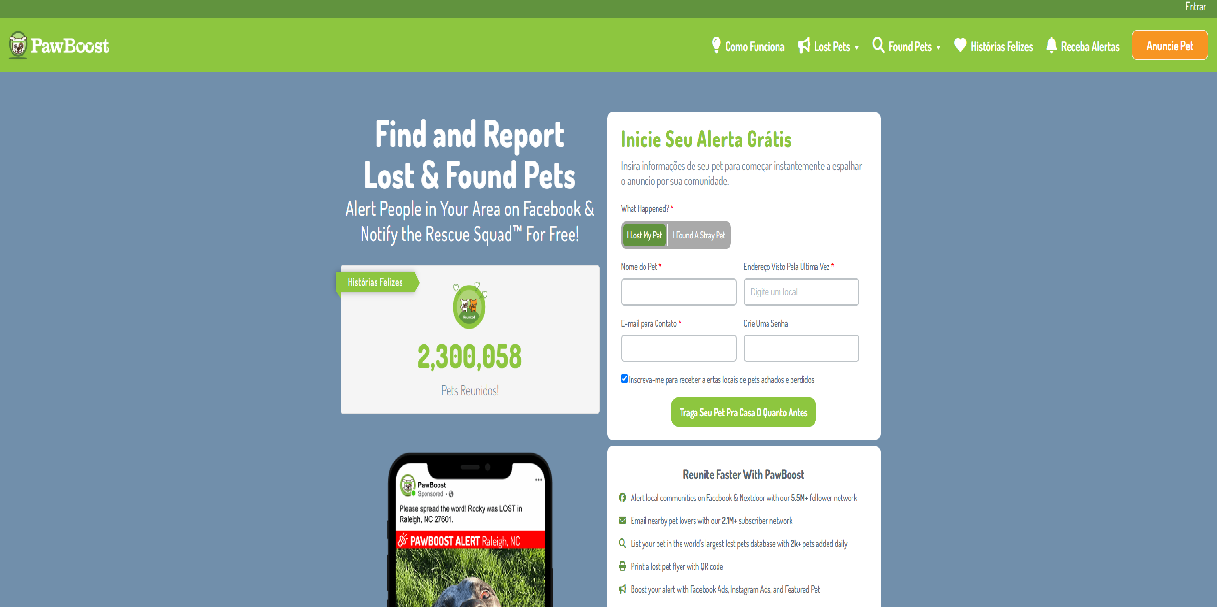
\includegraphics[width=0.90\textwidth]{imagens/01_pesquisa/figura04_pawboost.png}
    \fonte{PawBoost (2026)}
\end{figure}

A interface principal da plataforma (Figura~\ref{fig:pawboost}) estrutura-se com uma barra superior em tom verde que abriga o logotipo, atalhos de navegação (``Como Funciona'', ``Lost Pets'', ``Found Pets'', ``Histórias Felizes'', ``Receba Alertas'') e o botão alaranjado de chamada à ação ``Anuncie Pet''. No canto superior direito, há o link para autenticação (``Entrar''). Na lateral esquerda, visualiza-se a chamada de impacto ``Find and Report Lost \& Found Pets'', acompanhada pelo contador de impacto comunitário (``2,300,058 Pets Reunidos!'') e uma maquete de smartphone demonstrando o formato de alerta geolocalizado compartilhado no Facebook. Na lateral direita, destaca-se o cartão com formulário direto ``Inicie Seu Alerta Grátis'', contendo botões de seleção de ocorrência (``I Lost My Pet'' e ``I Found A Stray Pet''), campos para nome do pet, último endereço visto, e-mail para contato, senha e o botão verde de submissão ``Traga Seu Pet Pra Casa O Quanto Antes'', acompanhado pela lista dos recursos da rede.

Entre os pontos fortes, destacam-se a postagem automatizada em páginas de redes sociais, alertas por e-mail e notificações móveis para voluntários locais. Contudo, a plataforma apresenta fortes barreiras para uso no Brasil: sua segmentação territorial é desenhada para códigos postais norte-americanos e os planos pagos de impulsionamento demandam cobrança em moeda estrangeira (dólar americano), restringindo o acesso financeiro da população local.

\noindent\textbf{AlertPet:} Iniciativa nacional estruturada como portal web que atua no modelo de ``carro de som digital'', intermediando campanhas patrocinadas de busca regional (Figura~\ref{fig:alertpet}).

\begin{figure}[H]
    \centering
    \caption{Interface da plataforma AlertPet}
    \label{fig:alertpet}
    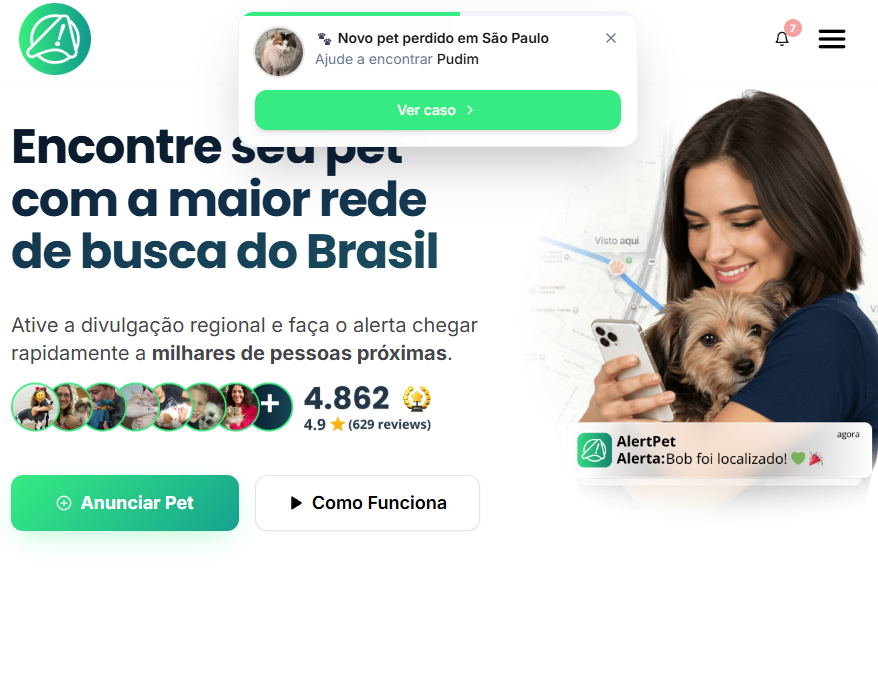
\includegraphics[width=0.90\textwidth]{imagens/01_pesquisa/figura05_alertpet.png}
    \fonte{AlertPet (2026)}
\end{figure}

Conforme apresentado na Figura~\ref{fig:alertpet}, a página inicial organiza-se com um cabeçalho limpo contendo o logotipo no canto superior esquerdo, um card flutuante centralizado que simula uma notificação em tempo real (``Novo pet perdido em São Paulo -- Ajude a encontrar Pudim'' acompanhado de foto e botão ``Ver caso'') e ícones de sino de alertas e menu hamburguer. No quadrante esquerdo inferior, destaca-se o título de grande porte ``Encontre seu pet com a maior rede de busca do Brasil'', acompanhado por dados de prova social com avatares de tutores (``4.862 casos'' e nota ``4.9 com 629 avaliações''), o botão verde de ação primária ``+ Anunciar Pet'' e o botão secundário ``Como Funciona''. Na composição visual da direita, exibe-se uma tutora segurando seu cão e celular, sobreposta por um recorte de mapa indicando o ponto de sumiço (``Visto aqui'') e uma notificação instantânea simulada (``AlertPet Alerta: Bob foi localizado!'').

A proposta central do \textit{AlertPet} consiste na criação profissional de cartazes digitais e na veiculação de campanhas pagas altamente geolocalizadas em redes sociais no raio onde o animal sumiu, com envio de relatórios formais de métricas. Contudo, operando prioritariamente como um serviço comercial de mídia paga, a ferramenta não disponibiliza um aplicativo móvel integrado, não conta com mapa interativo gratuito com GPS em tempo real e condiciona o alcance das buscas à contratação de pacotes comerciais.

\noindent\textbf{Pet911:} Plataforma de abrangência internacional com versão dedicada ao público brasileiro, focada na centralização de anúncios de achados e perdidos de animais domésticos (Figura~\ref{fig:pet911}).

\begin{figure}[H]
    \centering
    \caption{Interface da plataforma Pet911}
    \label{fig:pet911}
    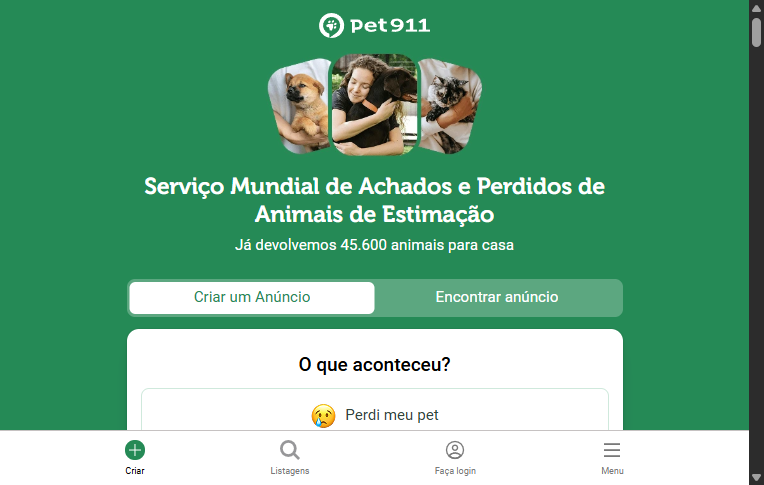
\includegraphics[width=0.90\textwidth]{imagens/01_pesquisa/figura06_pet911.png}
    \fonte{Pet911 (2026)}
\end{figure}

A interface inicial do Pet911 (Figura~\ref{fig:pet911}) adota uma composição visual mobile-first centrada na cor verde esmeralda. No topo, destaca-se o logotipo acompanhado por três molduras fotográficas circulares exibindo tutores e animais acolhidos. Abaixo, figura a chamada central ``Serviço Mundial de Achados e Perdidos de Animais de Estimação'', acompanhada pela métrica de alcance ``Já devolvemos 45.600 animais para casa''. O sistema disponibiliza duas abas superiores para alternância rápida de objetivo (o botão ativo em fundo branco ``Criar um Anúncio'' e o botão semitransparente ``Encontrar anúncio''), seguido por um cartão de triagem inicial com o título ``O que aconteceu?'' e o botão de acionamento ilustrado ``Perdi meu pet''. Na extremidade inferior, fixa-se uma barra de navegação com quatro ícones funcionais: ``+ Criar'', ``Listagens'', ``Faça login'' e ``Menu''.

Como pontos positivos, o Pet911 oferece ampla base de dados, fluxo simplificado de cadastro preliminar e geração automática de cartazes digitais. No entanto, o sistema apresenta carências expressivas na camada interativa: as buscas dependem de listagens tabulares por cidades, não havendo navegação dinâmica em mapa com traçado de rotas por GPS em tempo real, nem canal privativo de troca de mensagens instantâneas, além de condicionar o impulsionamento comunitário a pacotes tarifados.

\vspace{0.3cm}
\begin{table}[H]
\centering
\phantomsection\label{quadro:similares}
\small
\renewcommand{\arraystretch}{1.25}
\begin{tabular}{|>{\raggedright\arraybackslash}p{2.2cm}|>{\raggedright\arraybackslash}p{3.3cm}|>{\raggedright\arraybackslash}p{4.5cm}|>{\raggedright\arraybackslash}p{4.0cm}|}
\hline
\multicolumn{4}{|c|}{\textbf{Quadro 1: Análise Comparativa dos Sistemas Similares}} \\ \hline
\textbf{Nome} & \textbf{Definição} & \textbf{Funcionalidades} & \textbf{Pontos Positivos} \\ \hline
\textbf{Viu Meu Pet} & Plataforma web e móvel nacional para cadastro, busca e divulgação de animais perdidos e encontrados. & Cadastro nos achados e perdidos e Facebook, gerador de imagens para redes, cartazes com QR Code para impressão e cruzamento automático por IA, além de serviços pagos (anúncio em destaque, impulsionamento e carro de som). & Grande visibilidade no Brasil, variedade de ferramentas visuais gratuitas (cartazes e IA) e opções escaláveis para ampliar o alcance do resgate. \\ \hline
\textbf{PawBoost} & Plataforma internacional (web e móvel) voltada a alertas rápidos e engajamento comunitário em resgates. & Postagem em páginas locais do Facebook, alertas por e-mail e push para voluntários (\textit{Rescue Squad}™), mural de busca e gerador de cartazes, com opção de anúncios patrocinados no Facebook. & Grande rede comunitária de voluntários, automação de alertas para grupos locais e notificações diretas no celular. \\ \hline
\textbf{AlertPet} & Serviço nacional baseado em portal web que atua como um ``carro de som digital'', intermediando campanhas de busca. & Criação de cartazes digitais pela equipe, veiculação de anúncios geolocalizados nas redes sociais no raio do sumiço, relatórios de métricas (Reportei) e suporte via WhatsApp. & Alcance regional rápido que independe da rede de contatos pessoal do tutor, segmentação geográfica profissional e relatórios formais de desempenho. \\ \hline
\textbf{Pet911} & Plataforma web e móvel internacional (com versão no Brasil) de achados e perdidos de animais domésticos. & Cadastro simplificado de ocorrências, busca por listagem territorial, geração de cartazes para impressão e planos de divulgação patrocinada paga (redes sociais e e-mails). & Ampla base de registros internacionais, interface mobile simplificada, processos rápidos de publicação inicial e suporte a alertas comunitários. \\ \hline
\end{tabular}
\fonte{Autoria própria (2026)}
\end{table}

\subsection{Metodologia de Desenvolvimento de Software}

A construção do aplicativo exigiu uma forma ágil de trabalho, capaz de transformar as ideias da pesquisa em um aplicativo funcional, estável e fácil de usar. Como explicam Pressman e Maxim (2021) e Valente (2023), o desenvolvimento moderno de aplicativos para celular precisa de flexibilidade para receber melhorias contínuas, evitando modelos rígidos que deixam os testes apenas para o final do projeto.

\subsubsection{Abordagem Ágil e Ciclo de Vida Incremental}

Adotou-se o modelo de desenvolvimento em partes (incremental e iterativo) (VALENTE, 2023). Nesse modelo, o aplicativo não é construído todo de uma vez; em vez disso, cada funcionalidade é planejada, programada e testada passo a passo. 

O primeiro incremento concentrou-se na infraestrutura de segurança e persistência (telas de autenticação, cadastro e sessão no Supabase Auth). O segundo incremento estabeleceu o núcleo geográfico da aplicação (feed de publicações e mapa interativo com GPS via Expo Location). O terceiro incremento abrangeu a criação e edição de ocorrências de animais com upload otimizado de fotografias. O quarto incremento incorporou os recursos de comunicação privativa (chat em tempo real via WebSockets). Por fim, o quinto incremento integrou recursos complementares de utilidade pública: a geração de cartazes digitais com código QR para impressão e o Perfil Digital do Pet com código QR para identificação preventiva do animal.

\subsubsection{O Método Visual Kanban e a Gestão de Tarefas no Trello}

Para assegurar o ritmo contínuo de produção e a rastreabilidade das atividades, adotou-se o método visual Kanban, operacionalizado através da plataforma de gestão de projetos Trello (TRELLO, 2026). A rotina de trabalho apoiou-se em três princípios essenciais: a visualização contínua de todo o fluxo de trabalho por meio de cartões descritivos contendo requisitos claros, a limitação estrita do trabalho em andamento (Work in Progress) para manter o foco na conclusão e validação de cada parte antes de abrir novas demandas, e o gerenciamento ativo do fluxo de produção para evitar retrabalhos e assegurar o cumprimento dos prazos acadêmicos.

Na prática, o quadro no Trello foi estruturado em cinco etapas sequenciais de controle. O fluxo iniciava-se no Backlog Geral, que reunia todos os requisitos funcionais e técnicos derivados da pesquisa inicial. Em seguida, as tarefas priorizadas para execução imediata eram transferidas para a lista A Fazer. Durante a fase de escrita de código-fonte no editor ou modelagem de diagramas, os cartões permaneciam na lista Em Andamento. Uma vez concluída a implementação, a funcionalidade avançava para Em Testes e Revisão, onde passava por inspeções de interface e testes em dispositivos físicos. Por fim, após a validação completa e o versionamento do código no GitHub, a atividade era finalizada na coluna Concluído.

\subsubsection{Etapas do Processo de Desenvolvimento}

O projeto percorreu quatro etapas sistemáticas ao longo do ciclo de desenvolvimento. A primeira etapa correspondeu à concepção e ao levantamento de requisitos, na qual as respostas do questionário com a comunidade e a análise das ferramentas concorrentes foram consolidadas na definição de 43 requisitos funcionais e 14 requisitos não funcionais, apresentados no Capítulo 4.

A segunda etapa compreendeu a modelagem conceitual e o projeto de interface, englobando a criação dos diagramas de casos de uso e classes no software Astah UML (ASTAH, 2026), a estruturação do modelo relacional de banco de dados e o desenho iterativo das telas e da identidade visual na ferramenta Figma (FIGMA, 2026).

A terceira etapa consistiu na implementação e codificação modular do sistema, com a escrita do código-fonte em TypeScript no Visual Studio Code, adotando a biblioteca React Native (REACT NATIVE, 2026) e o ecossistema Expo (EXPO, 2026) na camada cliente, e a plataforma Supabase (SUPABASE, 2026) para serviços de autenticação, banco de dados PostgreSQL e armazenamento em nuvem, com controle de versão no Git e GitHub (apresentados nos Capítulos 5 e 6).

Por fim, a quarta etapa envolveu os testes, a validação técnica e a avaliação de usabilidade da aplicação, abrangendo a execução de testes funcionais de caixa-preta para conferência das regras operacionais e a aplicação prática do protocolo internacional System Usability Scale com 20 voluntários, cujos resultados são detalhados no Capítulo 7.

A união entre a pesquisa com os usuários, a organização pelo método Kanban e as boas práticas de engenharia de software sustentou a construção de uma aplicação estável e eficiente. O Capítulo 4 apresenta em detalhes os requisitos e os modelos conceituais do sistema WeFIND.
\clearpage
